\documentclass[tikz]{standalone}

\usepackage[latin1]{inputenc}
\usepackage{tikz}

% GNUPL
\begin{document}
\pagestyle{empty}


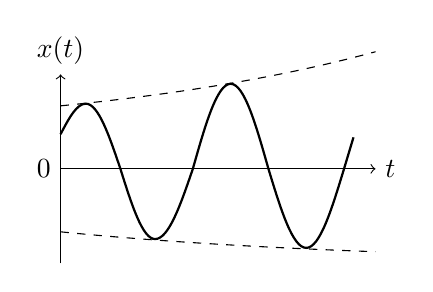
\begin{tikzpicture}[scale=0.4]
    %\draw[very thin,color=gray] (-1,1.1) grid (3.9,3.9);
    \draw[->] (0,0) -- (10,0) node[right] {$t$};
    \draw[->] (0,-3) -- (0,3) node[above] {$x(t)$};
    \draw [thick] (0,1.1) sin (0.8,2.07) cos (1.9,0) sin (3, -2.23) cos (4.2,0) sin (5.4, 2.7) cos (6.6, 0) sin (7.8, -2.51) cos (9, 0) -- (9.3, 1);
    \draw [black, dashed, domain=0:10,samples=200] plot (\x,  {exp(\x/10)+1});
    \draw [black, dashed, domain=0:10,samples=200] plot (\x,  {exp(-\x/10)-3});
    \coordinate [label=left:$0$] (0) at (0,0);


\end{tikzpicture}


\end{document}